\documentclass{article}\usepackage[]{graphicx}\usepackage[]{color}
%% maxwidth is the original width if it is less than linewidth
%% otherwise use linewidth (to make sure the graphics do not exceed the margin)
\makeatletter
\def\maxwidth{ %
  \ifdim\Gin@nat@width>\linewidth
    \linewidth
  \else
    \Gin@nat@width
  \fi
}
\makeatother

\definecolor{fgcolor}{rgb}{0.345, 0.345, 0.345}
\newcommand{\hlnum}[1]{\textcolor[rgb]{0.686,0.059,0.569}{#1}}%
\newcommand{\hlstr}[1]{\textcolor[rgb]{0.192,0.494,0.8}{#1}}%
\newcommand{\hlcom}[1]{\textcolor[rgb]{0.678,0.584,0.686}{\textit{#1}}}%
\newcommand{\hlopt}[1]{\textcolor[rgb]{0,0,0}{#1}}%
\newcommand{\hlstd}[1]{\textcolor[rgb]{0.345,0.345,0.345}{#1}}%
\newcommand{\hlkwa}[1]{\textcolor[rgb]{0.161,0.373,0.58}{\textbf{#1}}}%
\newcommand{\hlkwb}[1]{\textcolor[rgb]{0.69,0.353,0.396}{#1}}%
\newcommand{\hlkwc}[1]{\textcolor[rgb]{0.333,0.667,0.333}{#1}}%
\newcommand{\hlkwd}[1]{\textcolor[rgb]{0.737,0.353,0.396}{\textbf{#1}}}%
\let\hlipl\hlkwb

\usepackage{framed}
\makeatletter
\newenvironment{kframe}{%
 \def\at@end@of@kframe{}%
 \ifinner\ifhmode%
  \def\at@end@of@kframe{\end{minipage}}%
  \begin{minipage}{\columnwidth}%
 \fi\fi%
 \def\FrameCommand##1{\hskip\@totalleftmargin \hskip-\fboxsep
 \colorbox{shadecolor}{##1}\hskip-\fboxsep
     % There is no \\@totalrightmargin, so:
     \hskip-\linewidth \hskip-\@totalleftmargin \hskip\columnwidth}%
 \MakeFramed {\advance\hsize-\width
   \@totalleftmargin\z@ \linewidth\hsize
   \@setminipage}}%
 {\par\unskip\endMakeFramed%
 \at@end@of@kframe}
\makeatother

\definecolor{shadecolor}{rgb}{.97, .97, .97}
\definecolor{messagecolor}{rgb}{0, 0, 0}
\definecolor{warningcolor}{rgb}{1, 0, 1}
\definecolor{errorcolor}{rgb}{1, 0, 0}
\newenvironment{knitrout}{}{} % an empty environment to be redefined in TeX

\usepackage{alltt}
\usepackage{parskip}
\usepackage{amsmath}
\usepackage{lineno}
\usepackage{enumitem}
\usepackage{float}
\usepackage[left=1in,right=1in,top=1in,bottom=1in]{geometry}

\newcommand\ddfrac[2]{\frac{\displaystyle #1}{\displaystyle #2}}

\linenumbers

\title{Problem Set 3}
\author{Carrie Kathlyn Townley Flores, Filipe Recch, Kaylee Tuggle Matheny, \\ Klint Kanopka, Kritphong Mongkhonvanit \\ EDUC 252L}



\IfFileExists{upquote.sty}{\usepackage{upquote}}{}
\begin{document}
\maketitle

\section*{Shortish Answer}
\begin{enumerate}

\item Suppose that we have a test scaled with the Rasch model whose first 3 items have known difficulties -1, 0, and 1.5. An examinee with ability theta got the first item right, the second item right, and the third item wrong. Can you write the likelihood of observing this sequence of item responses as a function of theta?

The likelihood of getting each item right in the Rash model is given by:

$$ \frac{\epsilon^{\theta - b}}{1+\epsilon^{\theta - b}} $$ 

Therefore, each item's likelihood, considering its difficulty is as follows:
Item dif -1: $ \frac{\epsilon^{\theta + 1}}{1+\epsilon^{\theta + 1}} $ \\
Item dif 0: $ \frac{\epsilon^{\theta - 0}}{1+\epsilon^{\theta - 0}} $ \\
Item dif 1.5: $ 1 - \frac{\epsilon^{\theta - 1.5}}{1+\epsilon^{\theta - 1.5}} $ 

The chance of getting the specific sequence is the product of the probabilities of each item in the sequence. Hence, a 1-1-0 sequence has the probability equal to:

$$ \left(\frac{\epsilon^{\theta + 1}}{1+\epsilon^{\theta + 1}}\right) \times \left(\frac{\epsilon^{\theta - 0}}{1+\epsilon^{\theta - 0}} \right) \times \left(1 - \frac{\epsilon^{\theta - 1.5}}{1+\epsilon^{\theta - 1.5}} \right) $$

\item Can you plot this as a function of theta?

\begin{knitrout}
\definecolor{shadecolor}{rgb}{0.969, 0.969, 0.969}\color{fgcolor}\begin{figure}[H]

{\centering \includegraphics[width=\maxwidth]{figure/graph1-1} 

}

\caption[Probabilities as a function of theta]{Probabilities as a function of theta}\label{fig:graph1}
\end{figure}


\end{knitrout}

\item If theta=0.5, what is the likelihood of that response sequence?

\begin{knitrout}
\definecolor{shadecolor}{rgb}{0.969, 0.969, 0.969}\color{fgcolor}\begin{kframe}
\begin{alltt}
\hlstd{th}\hlkwb{<-}\hlnum{0.5}
\hlstd{p}\hlkwb{<-}\hlkwa{function}\hlstd{(}\hlkwc{b}\hlstd{)} \hlkwd{exp}\hlstd{(th}\hlopt{-}\hlstd{b)}\hlopt{/}\hlstd{(}\hlnum{1}\hlopt{+}\hlkwd{exp}\hlstd{(th}\hlopt{-}\hlstd{b))}
\hlkwd{round}\hlstd{(}\hlkwd{p}\hlstd{(}\hlopt{-}\hlnum{1}\hlstd{)}\hlopt{*}\hlkwd{p}\hlstd{(}\hlnum{0}\hlstd{)}\hlopt{*}\hlstd{(}\hlnum{1}\hlopt{-}\hlkwd{p}\hlstd{(}\hlnum{1.5}\hlstd{)),}\hlnum{3}\hlstd{)}
\end{alltt}
\begin{verbatim}
## [1] 0.372
\end{verbatim}
\end{kframe}
\end{knitrout}

\item If theta=0.5, what is the most likely response sequence given the known item difficulties? 

The probabilities of getting each item right is 0.82, 0.62 and 0.27, respectively for item difficulties of -1, 0, 1.5. Therefore, the most likely sequence is exactly 1-1-0.

\item At what value of theta does a response sequence of 1-1-0 (that is: they got the first and second items right and the third item wrong) become more likely than a response sequence of 1-0-0?

\begin{knitrout}
\definecolor{shadecolor}{rgb}{0.969, 0.969, 0.969}\color{fgcolor}\begin{figure}[H]

{\centering \includegraphics[width=\maxwidth]{figure/graph2-1} 

}

\caption[Probabilities as a function of theta]{Probabilities as a function of theta}\label{fig:graph2}
\end{figure}


\end{knitrout}

Considering that the only difference between the two sequeces is either the student got the second item right or wrong and that this specific item has difficulty $b = 0$, then getting 1-1-0 becames more likely at $\theta = 0$.

\item Returning to questions 1 and 2, can you plot the ``test information" as a function of theta (see Eqn 2-6 in Lord). 

To get the test information we need to sum over the all items information. In order to get the item information, we need to take the derivative with respect to $\theta$ of the probability of getting each item right. The ``test information" is as follows:

$$ \displaystyle\sum \ddfrac{\left(\ddfrac{\epsilon^{\theta+b}}{\left(\epsilon^{\theta}+\epsilon^{b}\right)^2}\right)^2}{\left(\ddfrac{\epsilon^{\theta-b}}{1+ \epsilon^{\theta-b}}\right) \left(1 - \ddfrac{\epsilon^{\theta-b}}{1 + \epsilon^{\theta-b}}\right)} $$

Using this formula, we get figure \ref{fig:graph3}.

\begin{knitrout}
\definecolor{shadecolor}{rgb}{0.969, 0.969, 0.969}\color{fgcolor}\begin{figure}[H]

{\centering \includegraphics[width=\maxwidth]{figure/graph3-1} 

}

\caption[Test information curve]{Test information curve}\label{fig:graph3}
\end{figure}


\end{knitrout}

\item Where is the function in \#6 maximized? What do you think this implies? 

In this case, the maximum is at 0.027.  This, in a sense, represents the ability score that the the test is best at measuring.  More specifically, the test is good at discerning between abilities near this value and worse at discerning between abilities far from this value.

\begin{knitrout}
\definecolor{shadecolor}{rgb}{0.969, 0.969, 0.969}\color{fgcolor}\begin{kframe}
\begin{verbatim}
## [1] 0.02702703
\end{verbatim}
\end{kframe}
\end{knitrout}

Since the value is very close to zero, it implies that $\theta$ will be
estimated most precisely when it is close to zero.

\item For an item response dataset of your choosing, consider the relationship between theta and the SE across the three IRT models for dichotomous items. How much of a difference does the choice of model have on the size of the error estimate?

First consider plots of the standard error vs. ability for the three IRT models, generated from the emp-rasch.txt data set used in lab:

\begin{knitrout}
\definecolor{shadecolor}{rgb}{0.969, 0.969, 0.969}\color{fgcolor}\begin{figure}[H]

{\centering 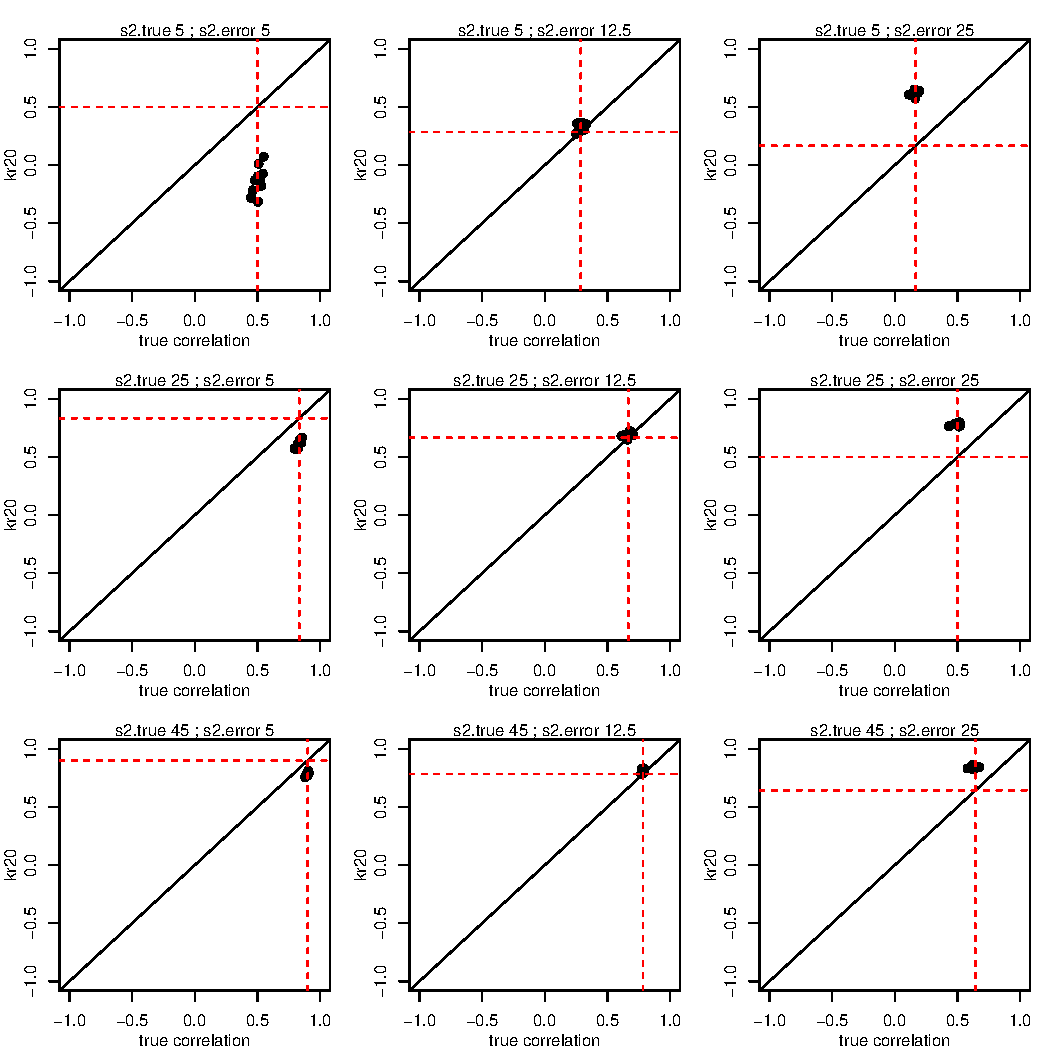
\includegraphics[width=\maxwidth]{figure/unnamed-chunk-4-1} 

}

\caption[Standard error as a function of ability]{Standard error as a function of ability}\label{fig:unnamed-chunk-41}
\end{figure}

\begin{figure}[H]

{\centering \includegraphics[width=\maxwidth]{figure/unnamed-chunk-4-2} 

}

\caption[Standard error as a function of ability]{Standard error as a function of ability}\label{fig:unnamed-chunk-42}
\end{figure}

\begin{figure}[H]

{\centering \includegraphics[width=\maxwidth]{figure/unnamed-chunk-4-3} 

}

\caption[Standard error as a function of ability]{Standard error as a function of ability}\label{fig:unnamed-chunk-43}
\end{figure}


\end{knitrout}

As you increase the number of estimated parameters in a model, the standard error, as a whole, decreases.  One interesting feature is the area of lowest standard error shifts between the models.  This is likely due to the change in estimated item difficulties as the models increase in complexity.  The reduction in standard error for more complex models makes sense, because the models ought to be able to fit the data better.  The most intersting part is the increase in error variance as the models become more complex.  This also makes sense, because there are more quantities being estimated for each item.  For the 3PL, especially, estimates of the guessing parameter are particularly unstable with low to moderate numbers of respondents, so this feature also makes sense.

\section*{Consulting Excercise}

A CTT approach would not be a responsible choice for the NDE to use with a high-stakes test. It would be easier and cheaper but much less meaningful. The only information we can get from a set of test scores in CTT is the total score of each of the test-takers. Any information we can get about the test items through CTT is population specific. As seen below, the data of 1000 test-takers organizes students by ability based only on their total scores, where theta is only meaningful in comparison to other test takers:

\centering
\begin{knitrout}
\definecolor{shadecolor}{rgb}{0.969, 0.969, 0.969}\color{fgcolor}

{\centering 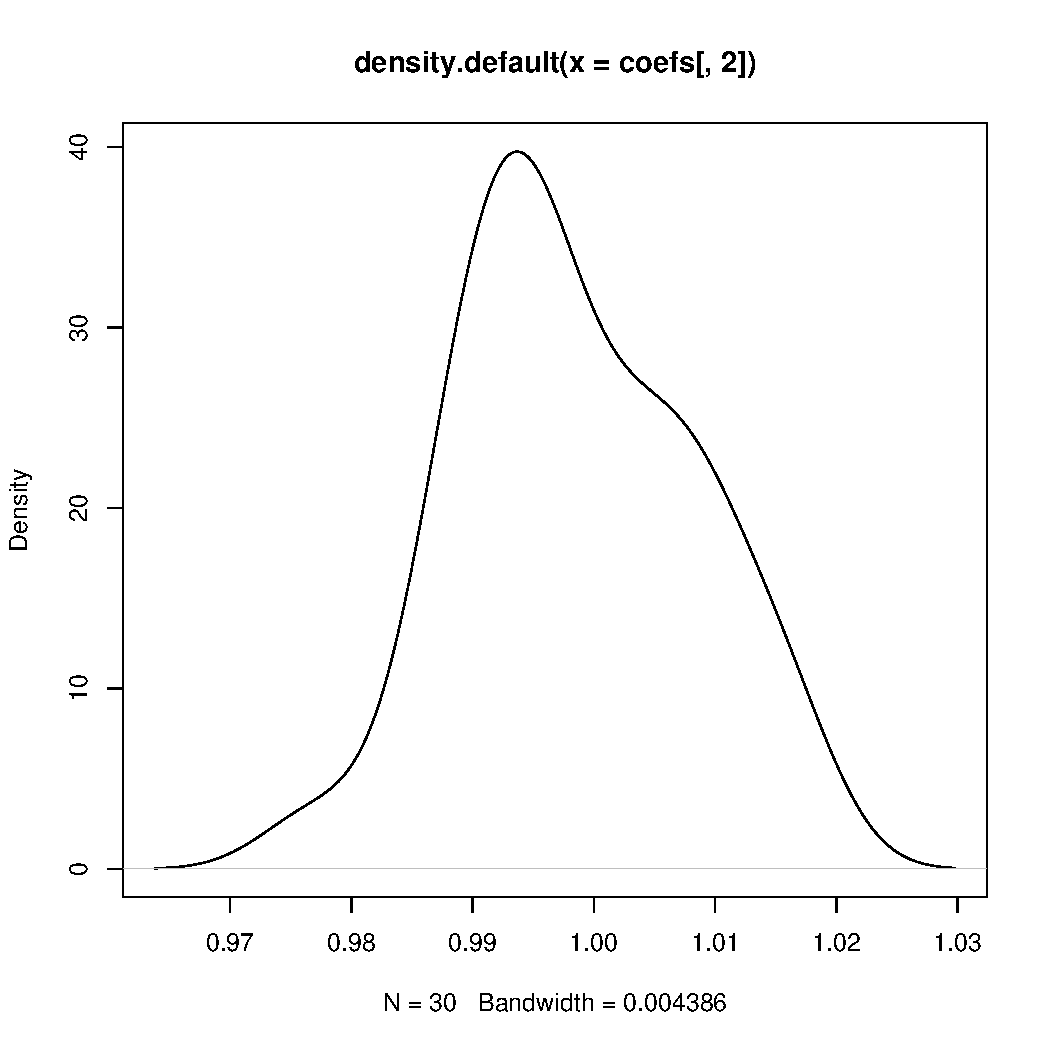
\includegraphics[width=.6\linewidth]{figure/unnamed-chunk-5-1} 

}




{\centering \includegraphics[width=.6\linewidth]{figure/unnamed-chunk-5-2} 

}



\end{knitrout}
\raggedright
This measure is only meaningful to the extent that our items are perfectly designed. In reality, items are not separated by even intervals, and they are not perfectly designed, so CTT is really lacking. 

As a hint of what measures of item quality we should be interested in, in the following chart, for each test item, test-takers' scores are compared to the percentage of students who answered that item correctly. This can give us information about which items are easier and which are harder. This chart is organized from the hardest items in the upper left, where almost no one answered correctly, to the easiest in the lower right, where at least some students at nearly all score levels answered correctly. This kind of analysis would tell us that we should consider dropping the first item because none of our students are answering it correctly, so it could be throwing off our analyses. This kind of analysis could also show us if some items are behaving in such a way that it does not follow an increasing pattern across student scores, in which case we should review whether or not that item has an element construct irrelevance, for instance. However, it could also be that the item is fine but our test-takers are not of high enough ability for that item. To determine this, other analyses are needed that CTT can not give us.

\centering
\begin{knitrout}
\definecolor{shadecolor}{rgb}{0.969, 0.969, 0.969}\color{fgcolor}

{\centering 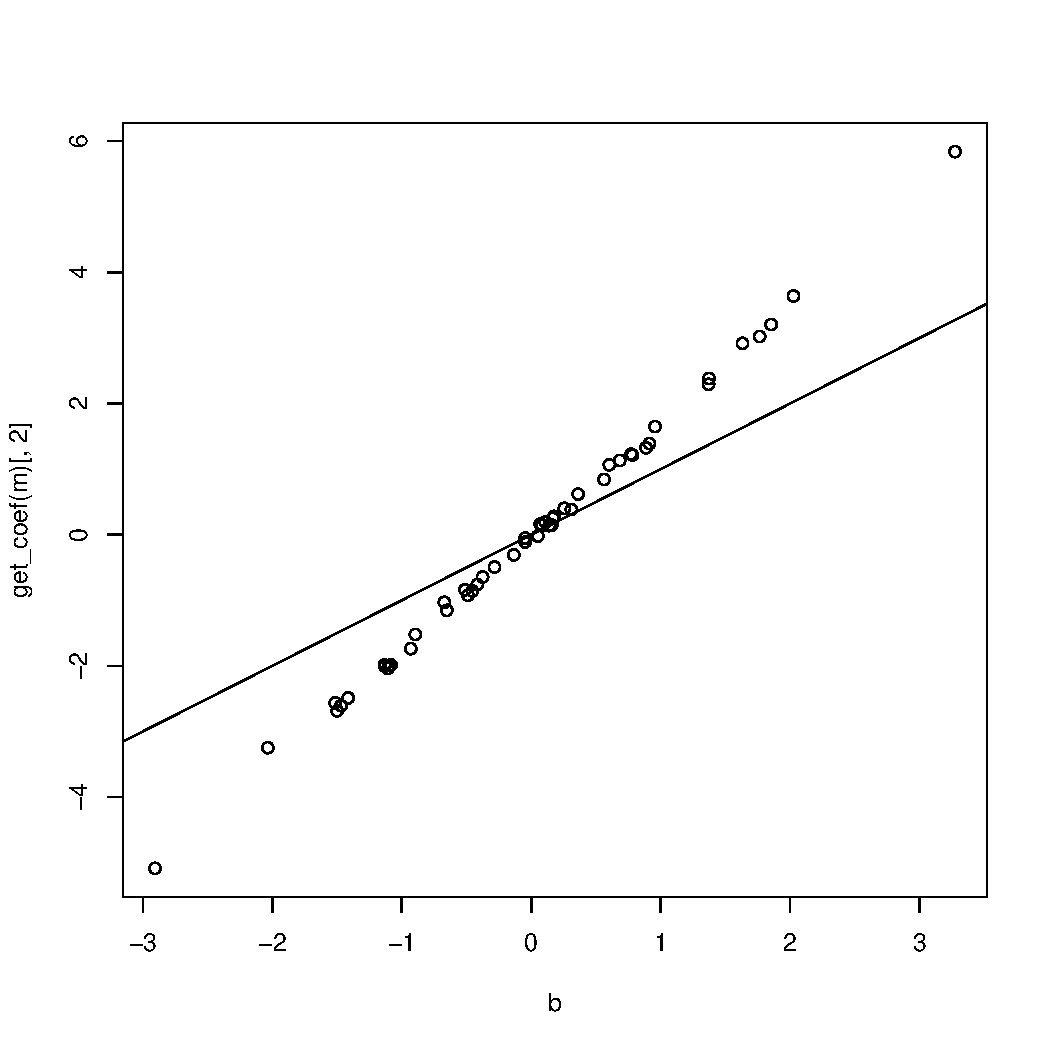
\includegraphics[width=.6\linewidth]{figure/unnamed-chunk-6-1} 

}



\end{knitrout}
\raggedright
In another visual that gives related information, here is a chart showing the correlation of patterns of test-taker responses as a function of the number of test-takers who answered that item correctly.

\centering
\begin{knitrout}
\definecolor{shadecolor}{rgb}{0.969, 0.969, 0.969}\color{fgcolor}

{\centering 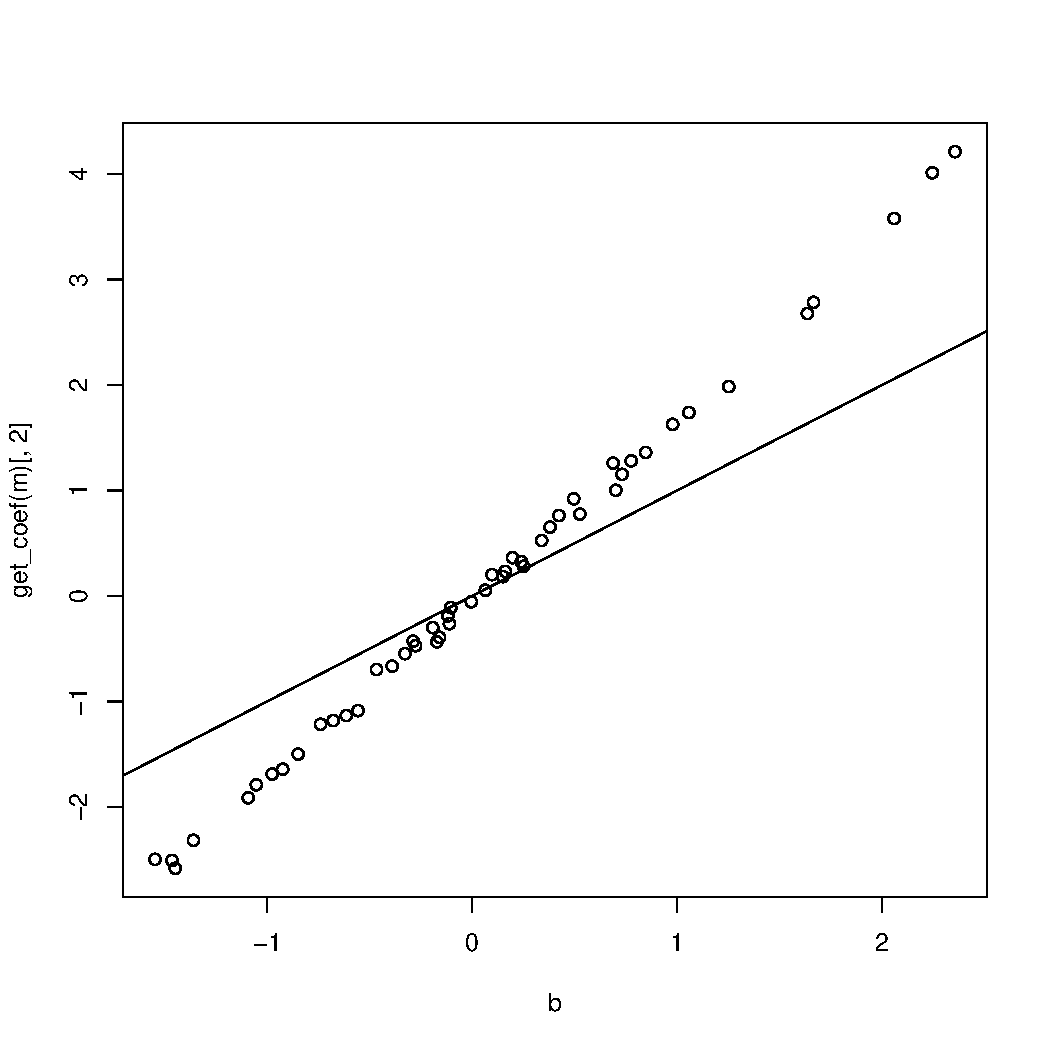
\includegraphics[width=.5\linewidth]{figure/unnamed-chunk-7-1} 

}



\end{knitrout}
\raggedright
This shows how the responses to each item correlate. 

In the next chart, we will take a different look at how item responses correlate with one another. White indicates no correlation, red means negative correlation, and blue means positive correlation. We can see that a few items are weakly correlated, and one item is negatively correlated with the other items. The line that is showing up with some red is the line associated with the item in the upper left corner of our earlier by-item chart. By showing that the trends in item responses to this item are not correlated with the trends in other items, it gives us further evidence that this item may have construct irrelevant variance. The lighter rows or columns also indicate some items that may be weaker and should be revisited. On the other hand, if items are showing up with very high correlations or dark blue squares, we will be alerted that we may have mirroring items that we need to cull.

\centering
\begin{figure}

\includegraphics[scale=0.45]{NDECorrelations}
\end{figure}
\raggedright
Using analyses like the ones above, we can also detect cheating across schools or within classrooms. If trends in student responses to certain items are widely variant from the rest of the population, we can flag a set of tests for further review.
\raggedright

What we can get out of each of these charts is that there is one outlying item that almost no one in our sample got correct, and that this pattern was not correlated with the patterns seen in any other items. This is useful information, but it is sample specific. It could be that this pattern is a function of something about this group of test-takers. Certainly the scatter of the correlation of patterns of test-item responses among questions that more test-takers answered correctly is population specific, and it may not look the same given another population. We want a model of measurement whose information is not specific to the population taking the test.
\raggedright

As the Rasch model can show us, abilities should probably be estimated as functions of attributes of the items. That would give us a measurement scale that does not change across populations. In the earlier by-item chart, we can see that the curves rise at different rates across test-taker score-levels, which indicates that some items are easier than others. With the Rasch model, we can numerically estimate item difficulty (or easiness), which can be used to give us better estimates of test-taker abilities. We can also get more information about the quality of our items this way.
\raggedright

A good test will have items that have difficulties that sufficiently cover the range of expected abilities such that they give us information at every place along the spectrum of abilities that we have interest in. CTT can not verify this.
\raggedright

In fact, by analyzing our data through the Rasch model, we find that most of the items fall between -2 and 2 standard deviations of average easiness, with one extreme outlier, as shown below.

\centering
\begin{knitrout}
\definecolor{shadecolor}{rgb}{0.969, 0.969, 0.969}\color{fgcolor}

{\centering 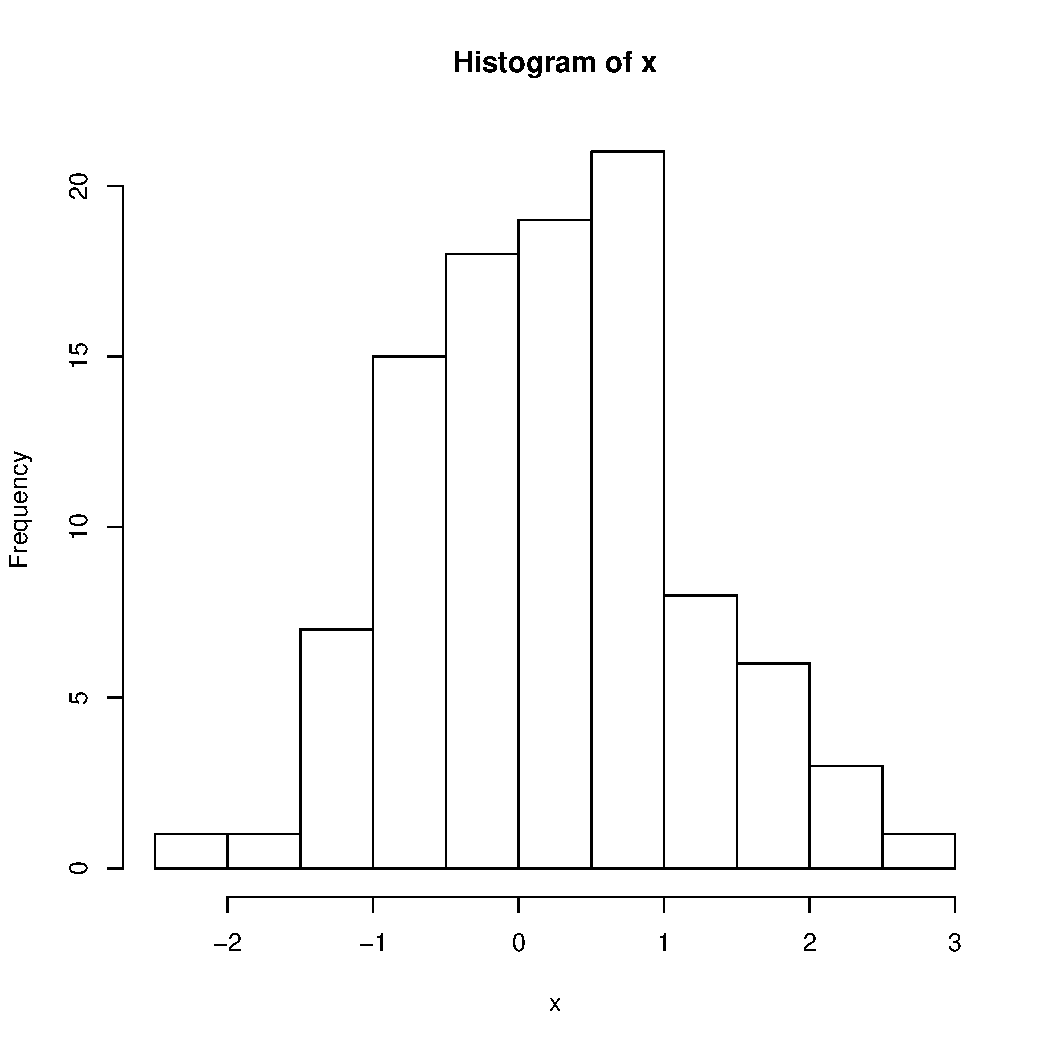
\includegraphics[width=.6\linewidth]{figure/unnamed-chunk-8-1} 

}



\end{knitrout}
\raggedright
This is an advantage over CTT in two ways. It lets us better analyze our test, and it gives us meaningful information about a single test-taker, apart from how they fare among other test-takers. In IRT, we can estimate a test-taker's ability based on the difficulty of the items that person answered correctly. Test-takers with the same sum score may be found to have different abilities, and the ranking from the Rasch model is more accurate that way. 

IRT also allows us to analyze test reliability by measuring Cronbach's alpha, which is a measure of internal consistency. In fact, the Rasch model shows us that our items are reliable. A score above .7 is generally considered good. This score only increases when we remove item 22, which we already sense is problematic.

\centering

\raggedright
Cronbach's alpha = 0.901 %this is printing alpha

Cronbach's alpha without item 22 = 0.902
\raggedright

Before we go much further into that explanation, I want to address the other argument, that we should switch to the even more computationally complex 3PL model. It is proposed that because this model actually gives us even more parameters with which to score our test-takers, it is superior to the Rasch model. Namely, the 3PL model lets us look at item discrimination, or how quickly the probability of getting a correct answer increases with respect to ability, and a guessing parameter that could theoretically correct scores for the possiblity of guessing on item answers. Taking into account item discrimination does give us more information at the ability levels associated with sharply discriminating items. However, the guessing parameter is very difficult to estimate, and overall, this model is not a huge improvement over the Rasch model, and I do not recommend its use. However, it is worth exploring what this model has to offer.

Now that we have laid the groundwork, we can start comparing CTT, the Rasch, and the 3PL models. In the following chart, you will see three bar graphs showing the distribution of abilities determined by each of the models. Below the diagonal, you can see regressions of the model in that column, as the x-axis, against the model in that row, as the y-axis, with ellipses noting one standard deviation in each direction around the mean. Above the diagonal, you will see Pearson correlation coefficients, which show that each of the models is similar, with the Rasch and 3PL nearly perfectly correlated. What you will note regarding the CTT model compared to the other two is that students given the same sum score, and therefore the same ability under CTT, are spread among a range of abilities in the other two models. This happens because the other two models are taking into account characteristics of the items themselves. You will also notice that while the range of abilities in the 3PL method provides a more normal-looking curve due to lowering some students' abilities after taking into account a guessing parameter, the measurement of the 3PL is otherwise very close to that of the Rasch model.

\centering
\begin{knitrout}
\definecolor{shadecolor}{rgb}{0.969, 0.969, 0.969}\color{fgcolor}\begin{kframe}


{\ttfamily\noindent\itshape\color{messagecolor}{\#\# EM cycles terminated after 500 iterations.}}\end{kframe}

{\centering 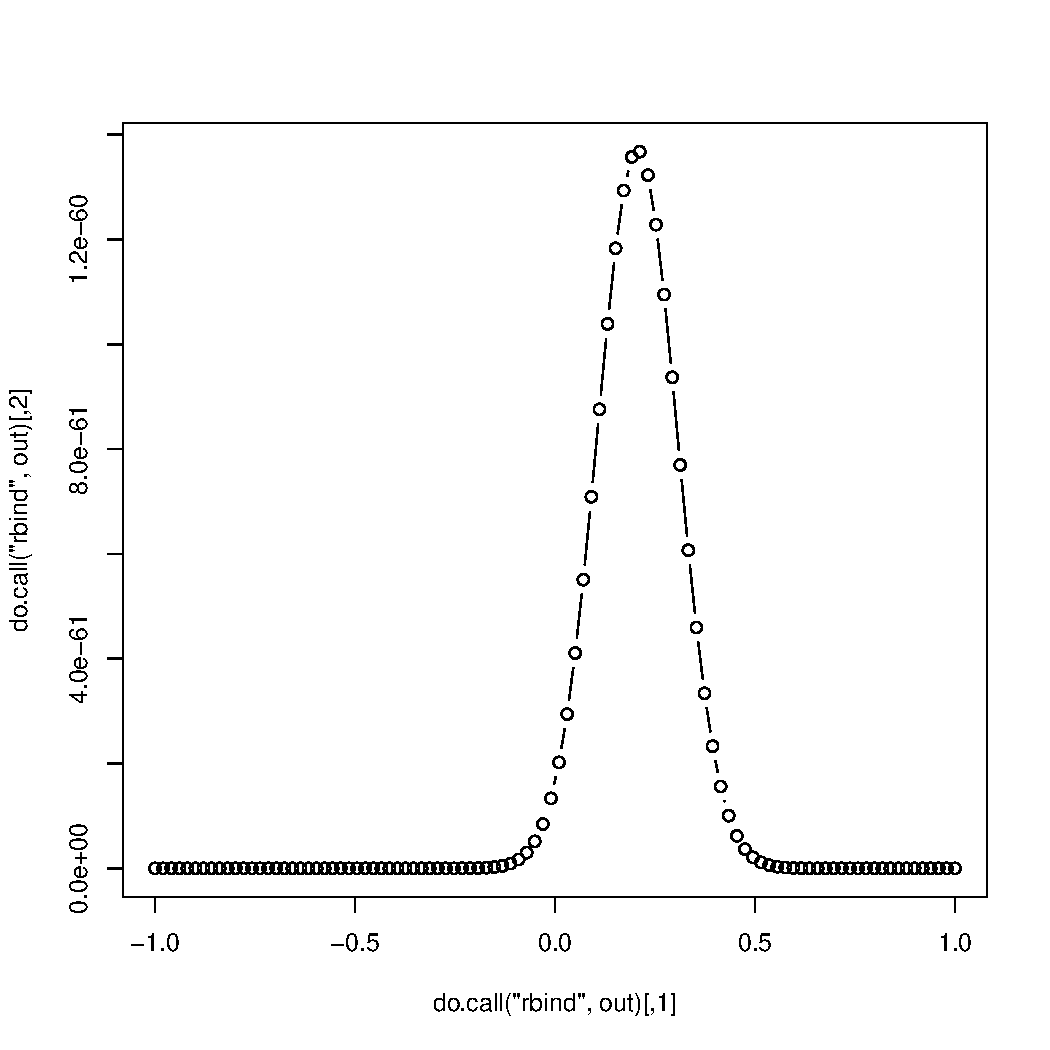
\includegraphics[width=.75\linewidth]{figure/unnamed-chunk-10-1} 

}



\end{knitrout}
\raggedright
The extra information offered by the guessing parameter in the 3PL method may be enticing, but it is actually cumbersome to compute accurately (For example, we can not do it with our small sample of 1000!). A guessing parameter is also an artifact of the test-takers rather than the test itself, and it varies among test-taking groups. We have to ask ourselves what we want out of the measurement device we choose. If we want a device that acts like a ruler, working the same way for every population, then we need to abandon the 3PL method.
\raggedright

In my effort to convince you, I will show you in more detail the differences among the models. 
In CTT, we have a discrete number of ability scores we can give test-takers, based on the number of items in the test. With IRT, ability scores fall in a continuum above and below the mean in a near normal distribution.

\centering
\begin{knitrout}
\definecolor{shadecolor}{rgb}{0.969, 0.969, 0.969}\color{fgcolor}

{\centering 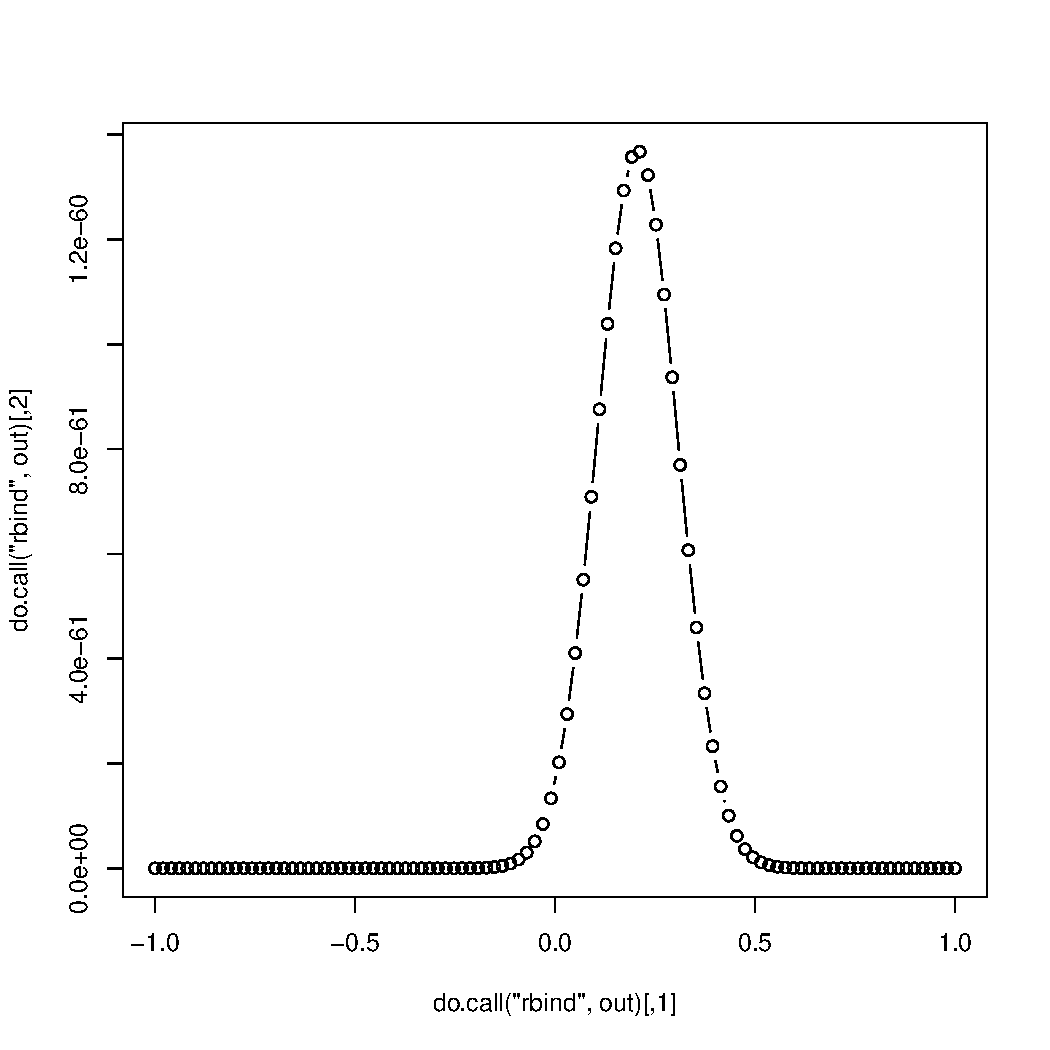
\includegraphics[width=.6\linewidth]{figure/unnamed-chunk-11-1} 

}



\end{knitrout}
\raggedright
Similarly, in the 2PL and the 3PL (shown here), abilities fall in a continuum. The outliers have near-perfect or near-imperfect scores.

\centering
\begin{knitrout}
\definecolor{shadecolor}{rgb}{0.969, 0.969, 0.969}\color{fgcolor}\begin{kframe}


{\ttfamily\noindent\itshape\color{messagecolor}{\#\# EM cycles terminated after 500 iterations.}}\end{kframe}

{\centering 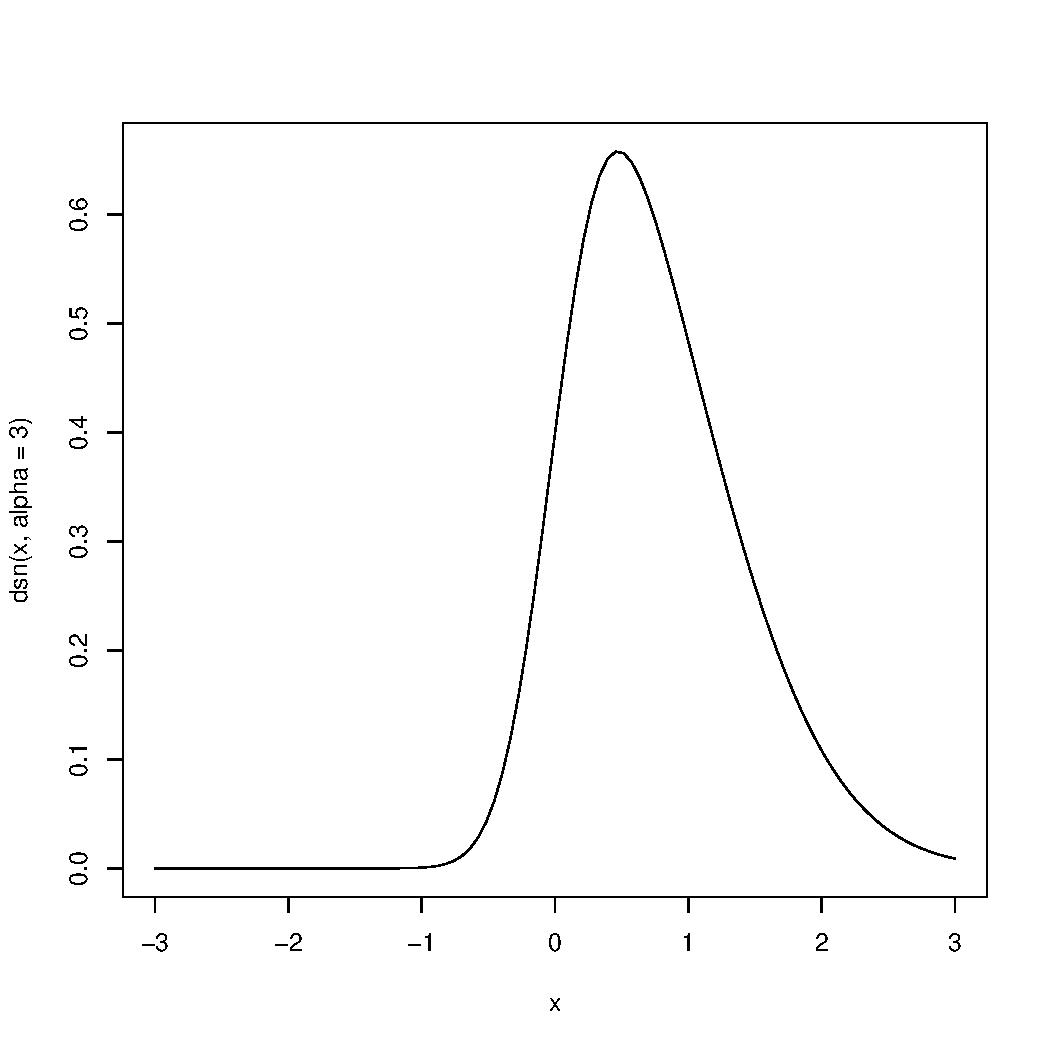
\includegraphics[width=.6\linewidth]{figure/unnamed-chunk-12-1} 

}



\end{knitrout}
\raggedright
It is important to note how the ability estimates change from model to model.

\centering
\begin{knitrout}
\definecolor{shadecolor}{rgb}{0.969, 0.969, 0.969}\color{fgcolor}\begin{kframe}


{\ttfamily\noindent\itshape\color{messagecolor}{\#\# EM cycles terminated after 500 iterations.}}\end{kframe}\begin{figure}[H]

{\centering 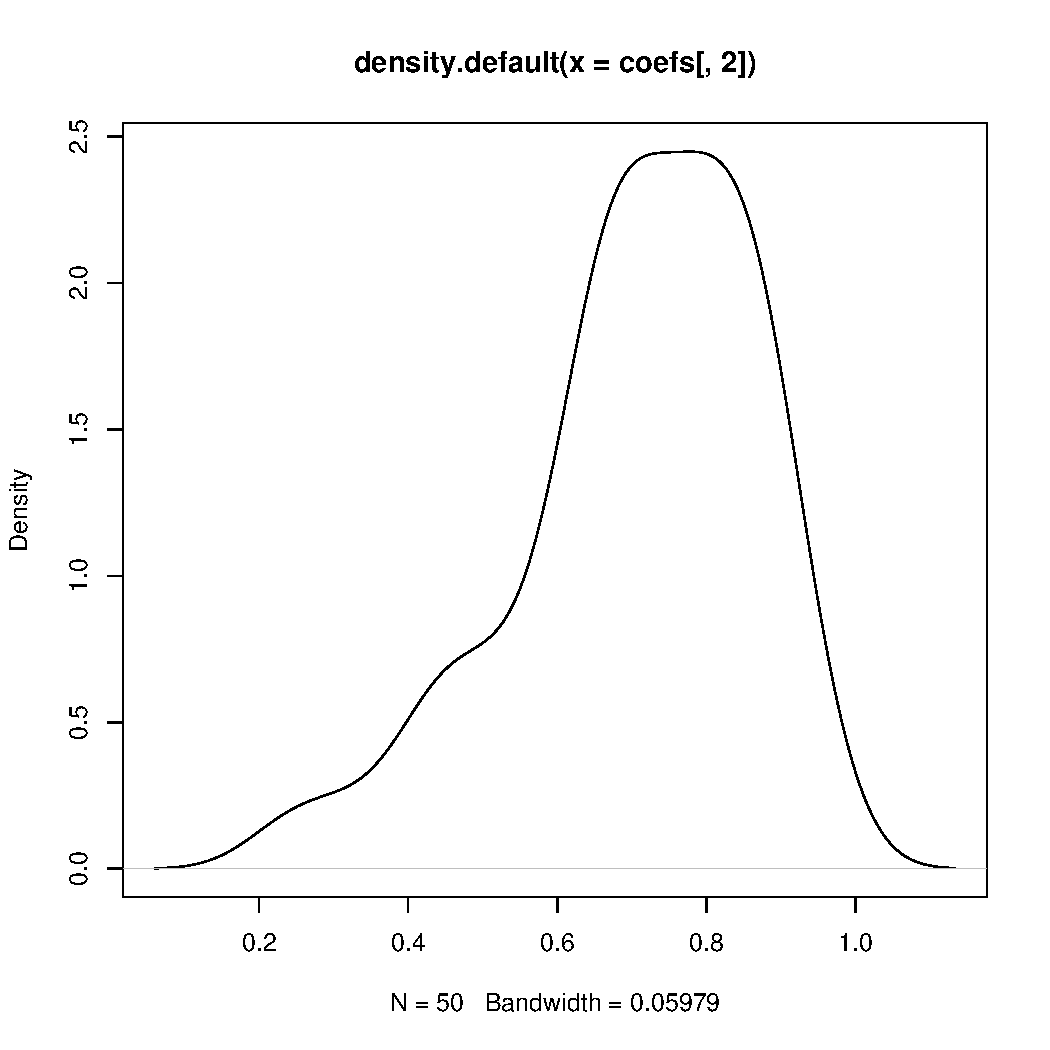
\includegraphics[width=.6\linewidth]{figure/unnamed-chunk-13-1} 

}

\caption[Distribution of changes in respondent ability measures between models]{Distribution of changes in respondent ability measures between models}\label{fig:unnamed-chunk-131}
\end{figure}

\begin{figure}[H]

{\centering 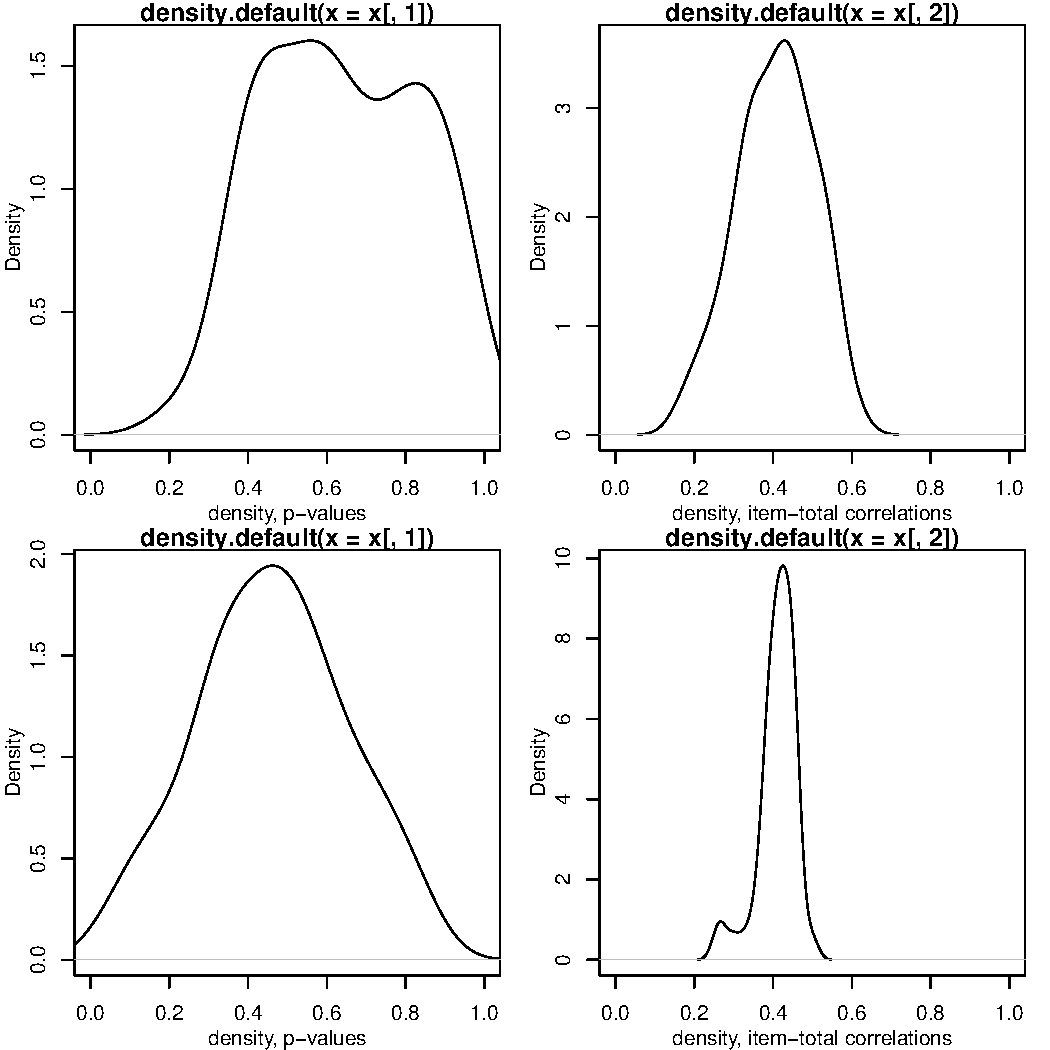
\includegraphics[width=.6\linewidth]{figure/unnamed-chunk-13-2} 

}

\caption[Distribution of changes in respondent ability measures between models]{Distribution of changes in respondent ability measures between models}\label{fig:unnamed-chunk-132}
\end{figure}

\begin{figure}[H]

{\centering \includegraphics[width=.6\linewidth]{figure/unnamed-chunk-13-3} 

}

\caption[Distribution of changes in respondent ability measures between models]{Distribution of changes in respondent ability measures between models}\label{fig:unnamed-chunk-133}
\end{figure}


\end{knitrout}
\raggedright
As you can see, most ability estimates do not change much from the Rasch to the 3PL model, and none increase by more than .5 standard deviations. A few more decrease in ability, but as you will see, this comes with caveats as the standard errors also increase and increase in variation at the low end of the 3PL model estimates. Also, in high-stakes testing, it is more harmful to make errors in scoring test-takers at too low abilities than too high abilities, so keeping the Rasch model over the 3PL model is not increasing the chance of doing harm. It is not to say that we should choose a model because it gives test-takers higher scores, but it is to say that if we do not trust the 3PL model fully, and if it is prone to more variance in error at the lower end, we have many reasons not to choose it.
\raggedright

These ability estimates depend on item characteristics determined by the models. The information we have about the test-takers at various ability levels is based on the amount of information the items give us. Along with the information curves above, we can look at Wright Maps to determine where we have the most information and where we are lacking information. Wherever we have the most information, the standard errors in our ability estimates will be lowest.

\centering
\begin{knitrout}
\definecolor{shadecolor}{rgb}{0.969, 0.969, 0.969}\color{fgcolor}

{\centering 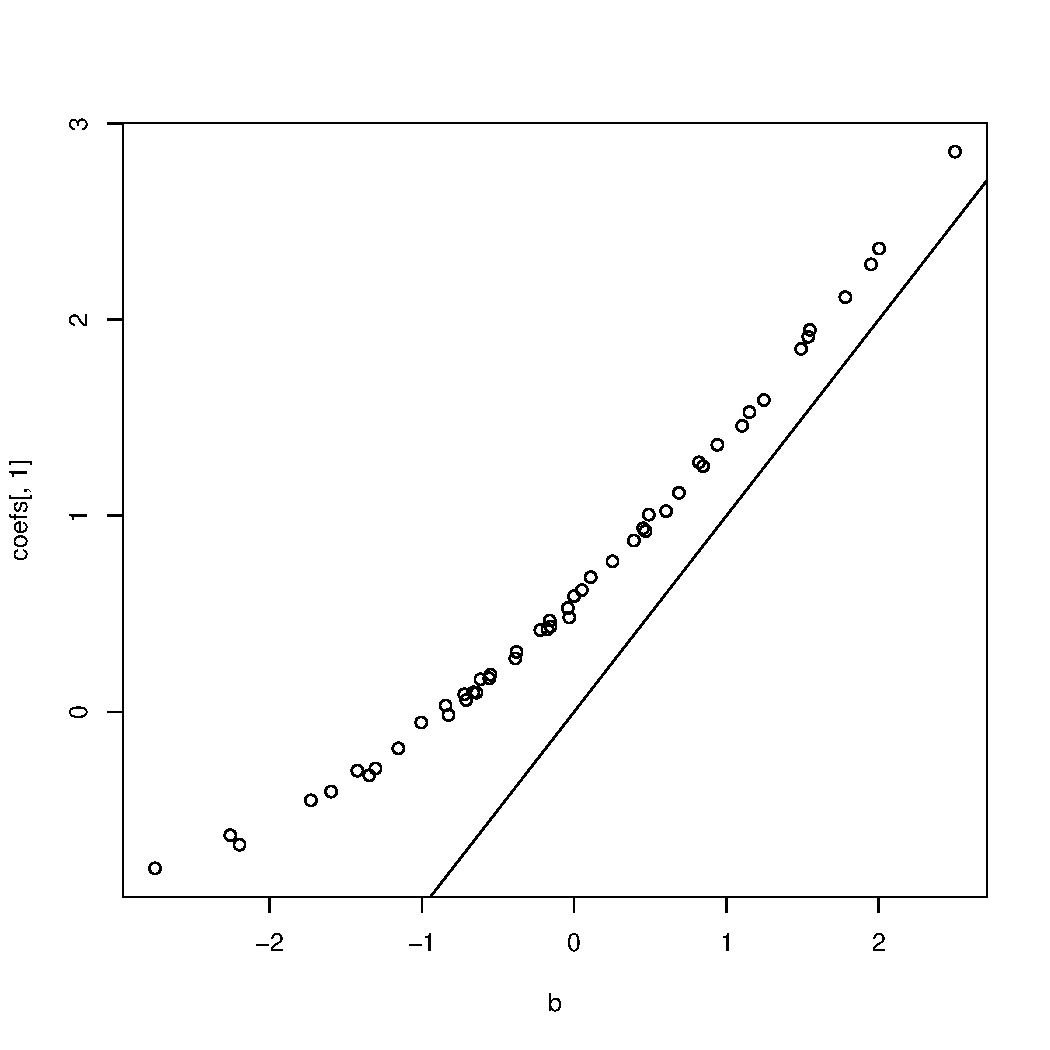
\includegraphics[width=\maxwidth]{figure/unnamed-chunk-14-1} 

}




{\centering \includegraphics[width=\maxwidth]{figure/unnamed-chunk-14-2} 

}



\end{knitrout}
\raggedright
This shows that we are missing information at the low end and the highest ends of abilities. Sure enough, this can be shown by the item information curves.

\raggedright
If we look at just the first five items in our sample, item information curves look like this:

\centering
\begin{knitrout}
\definecolor{shadecolor}{rgb}{0.969, 0.969, 0.969}\color{fgcolor}

{\centering \includegraphics[width=.6\linewidth]{figure/unnamed-chunk-15-1} 

}



\end{knitrout}
\raggedright
This shows that the first item offers the most information around -1, and the rest offer the most information around 0. If all of our items looked like one of these, we would want to know because these items do not give us much information about the students 1 standard deviation above the mean or 2 standard deviations below. 
\raggedright

If we look at all 40 items, we can analyze the whole sample test.

\centering
\begin{knitrout}
\definecolor{shadecolor}{rgb}{0.969, 0.969, 0.969}\color{fgcolor}

{\centering \includegraphics[width=.5\linewidth]{figure/unnamed-chunk-16-1} 

}



\end{knitrout}
\raggedright
The low discrimination of a few items, shown by the flatter information curves, indicate that while some items may not be throwing off our ability scores, they are not giving us much information about our test-takers' abilities either.
\raggedright

Based on this visual of the information each item is giving us, we can calculate where in the ability distribution the test is most meaningful.

\centering
\begin{knitrout}
\definecolor{shadecolor}{rgb}{0.969, 0.969, 0.969}\color{fgcolor}

{\centering \includegraphics[width=.5\linewidth]{figure/unnamed-chunk-17-1} 

}



\end{knitrout}
\raggedright
As you can see, we do not have a lot of information at the low or mid-high ranges, which tells us that we will have higher errors in our scores at these ranges.
\raggedright

This also shows us that we have some items that are so poorly discriminating, they may be worth replacing as they are not contributing greatly to our overall measurement goal.
\raggedright

It is interesting to note that the above example used item discrimination, which is a parameter in the 2PL and 3PL models, but not in the Rasch model. The 2PL model would tell us the discrimination of our items looks like this:

\centering
\begin{knitrout}
\definecolor{shadecolor}{rgb}{0.969, 0.969, 0.969}\color{fgcolor}\begin{kframe}


{\ttfamily\noindent\itshape\color{messagecolor}{\#\# EM cycles terminated after 500 iterations.}}\end{kframe}

{\centering \includegraphics[width=.6\linewidth]{figure/unnamed-chunk-18-1} 

}



\end{knitrout}
\raggedright
While this seems like important information, it does not actually affect the overall test information curve that much. As you can see in the test information curves, the Rasch model offers almost the same overall information as the 2PL model.

\centering

\raggedright
Unsurprisingly, the standard error curves mirror the information curves.

\centering
\begin{knitrout}
\definecolor{shadecolor}{rgb}{0.969, 0.969, 0.969}\color{fgcolor}\begin{figure}[H]

{\centering \includegraphics[width=.6\linewidth]{figure/unnamed-chunk-20-1} 

}

\caption[Standard error as a function of ability]{Standard error as a function of ability}\label{fig:unnamed-chunk-201}
\end{figure}

\begin{figure}[H]

{\centering \includegraphics[width=.6\linewidth]{figure/unnamed-chunk-20-2} 

}

\caption[Standard error as a function of ability]{Standard error as a function of ability}\label{fig:unnamed-chunk-202}
\end{figure}

\begin{figure}[H]

{\centering \includegraphics[width=.6\linewidth]{figure/unnamed-chunk-20-3} 

}

\caption[Standard error as a function of ability]{Standard error as a function of ability}\label{fig:unnamed-chunk-203}
\end{figure}


\end{knitrout}
\raggedright
As you can see, the 3PL method adds quite a bit of measurement error at the low end, especially with this set of items that is missing information at the low end, and with this sample size that is inappropriate for generating guessing parameters. The Rasch model is more appropriate for our purposes. 
\raggedright

Finally, we should ask whether or not the Rasch model has good fit, and we see that it does, with the exception of our one item that we already know to be faulty.

\centering
\begin{knitrout}
\definecolor{shadecolor}{rgb}{0.969, 0.969, 0.969}\color{fgcolor}

{\centering \includegraphics[width=\maxwidth]{figure/unnamed-chunk-21-1} 

}



\end{knitrout}
\raggedright
Given the wealth of information, reliability, model fit, and accuracy we can gain by using the Rasch model and the unsubstantial gains we sustain by moving to the computationally expensive 3PL model, I recommend that the NDE use the Rasch model in our analyses.

\end{enumerate}
\end{document}
